% - - -
% Capítulo 4
% - - -
\chapter{Método da Solução Proposta}
\label{chap:solucaoproposta}

\todo[inline]{\textbf{NOTA}: Deve-se apresentar a visão geral da solução proposta, neste capitulo você deve apresentar metodologia do trabalho ou procedimentos metodológicos – deve constar o instrumental, os métodos e as técnicas aplicados para a elaboração do trabalho.}

\section{Arquitetura}

\todo[inline]{\textbf{NOTA}: Deve-se apresentar uma visão geral da solução proposta, exemplo, usando uma Big Picture. Abaixo segue um \textbf{exemplo}.} 

A Figura~\ref{fig_bigpicture} apresenta uma visão geral da solução proposta que visa o desenvolvimento e análise de uma sistema de irrigação usando tecnologias de IoT.

\begin{figure}[h!]
    \caption{\label{fig_bigpicture}Como funciona o sistema de irrigação.}
	\begin{center}
	    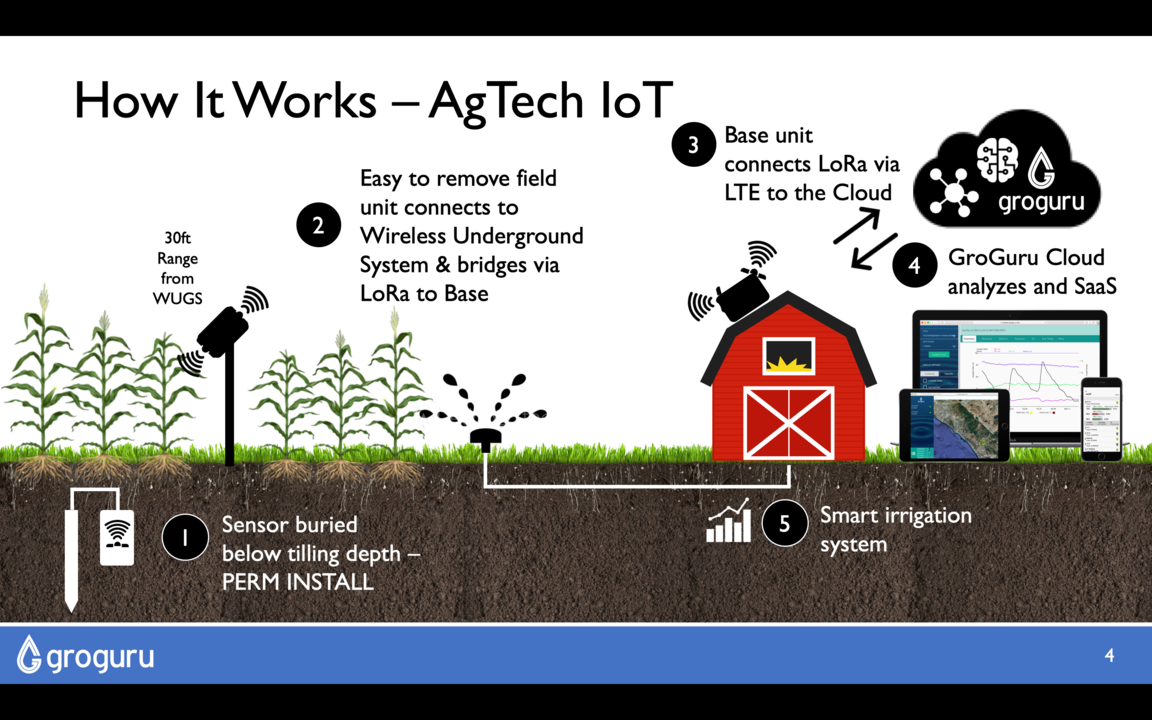
\includegraphics[scale=0.3]{images/bigpicture.png}
	\end{center}
	\legend{Fonte: Internet em \cite{groguru:2019}}
\end{figure}

\todo[inline]{\textbf{NOTA}: Nesta seção, também deve-se apresentar o fluxo da sua solução, ou seja, um diagrama contendo os artefatos de entrada e saída para cada etapa da solução proposta. Um modelo de digrama que pode ser utilizado é o BPMN (http://www.bpmn.org). Abaixo segue um \textbf{exemplo}.}

A Figura~\ref{fig_digflow} apresenta o fluxo de execução da solução proposta contendo suas respectivas entradas e artefatos gerados no modelo BPMN.

\begin{figure}[h!]
	\caption{\label{fig_digflow}Diagram de fluxo no modelo BPMN.}
	\begin{center}
	    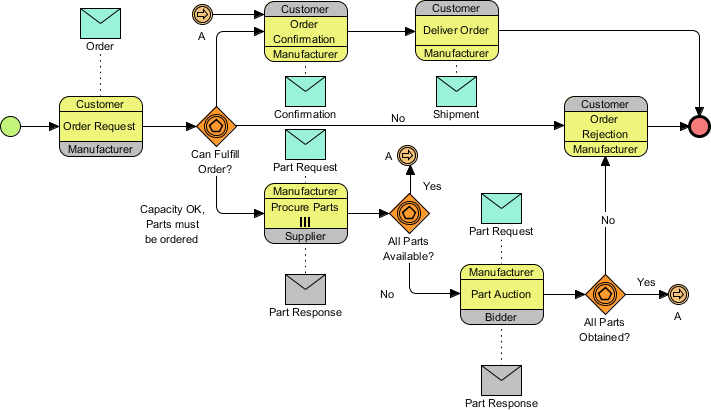
\includegraphics[scale=0.7]{images/34-final-business-process-diagram.png}
	\end{center}
	\legend{Fonte: Internet em \cite{bpmn:2019}}
\end{figure}


\section{Ferramentas e Implementações}

\todo[inline]{\textbf{NOTA}: Deve-se apresentar as ferramentas já pesquisadas que serão adotadas na solução propostas, bem como, explicar como as ferramentas serão correlacionadas. \textbf{Importante}, mencionar o nome da ferramenta, versão e onde pode ser encontrada, segue um pequeno \textbf{exemplo} de uso.}

A solução proposta será uma ferramenta de verificação de código implementada como um transformador de código escrita em C/C++ usando o \textit{framework} para compiladores LLVM~\footnote{https://llvm.org/} (v$6.0$)~\cite{Lattner:2004}. A solução utilizará como \textit{front-end} para programas escritos em C o Clang~\footnote{https://clang.llvm.org/} (v$6.0$)~\cite{Fandrey:2010} para gerar código LLVM-bitcode que será usado para a transformação de código. As ferramentas LibFuzzer~\cite{libfuzzer:2018} (v$6.0$) e KLEE~\cite{Cadar:2008:KUA} (v$2.0$) serão utilizadas para gerar entrada de testes para os códigos que serão analisados. Finalmente, o MetaSMT (v$4.rc2$) será usado como API para motores de solucionadores de satisfabilidade.


\section{Considerações Adicionais}

\todo[inline]{\textbf{NOTA}: Deve-se apresentar um visão geral em relação a construção da solução proposta. Analisar os pontos positivos e limitações da prototipação da prevista para a execução da solução.}